% book模板
% book模板.tex

\documentclass[12pt,UTF8]{ctexbook}

% 设置纸张信息。
\input{../../../common/page}

% 设置字体，并解决显示难检字问题。
\xeCJKsetup{AutoFallBack=true}
% 注意：ctexbook类已默认设置SimSun为CJKrmdefault
% 以下设置用于确保字体回退和扩展字体可用
% 仅设置扩展字体以避免与默认设置冲突
\setCJKfamilyfont{hei}{SimHei}
\setCJKfamilyfont{kai}{KaiTi}

% 目录 chapter 级别加点（.）。
\usepackage{titletoc}
\titlecontents{chapter}[0pt]{\vspace{3mm}\bf\addvspace{2pt}\filright}{\contentspush{\thecontentslabel\hspace{0.8em}}}{}{\titlerule*[8pt]{.}\contentspage}

% 支持目录点击跳转
\usepackage[colorlinks,linkcolor=blue,citecolor=blue,urlcolor=blue]{hyperref}

% 设置 part 和 chapter 标题格式。
\ctexset{
	part/name= {第,卷},
	part/number={\chinese{part}},
	chapter/name={第,篇},
	chapter/number={\arabic{chapter}}
}

% 图片相关设置。
\usepackage{graphicx}
\usepackage{float}
\graphicspath{{Images/}}

% 设置署名格式。
\newenvironment{shuming}{\hfill\zihao{4}}

% 注脚每页重新编号，避免编号过大。
\usepackage[perpage]{footmisc}

% 设置古文原文格式。
\newenvironment{yuanwen}{\bfseries\zihao{4}}

% 设置段落间距
\setlength{\parskip}{0.8em plus 0.2em minus 0.1em}

% 列表格式支持，列表项向右偏移。
\usepackage{enumitem}

% 数学公式支持
\usepackage{amsmath}

\title{\heiti\zihao{0} 题目}
\author{WangFei}
\date{\today}

\begin{document}

\maketitle
\tableofcontents

\frontmatter
\chapter{前言、序言}

\mainmatter

\part{基础理论}
\label{part:basics}

\chapter{无线电入门}
\label{chap:intro}

\section{电磁振荡与振荡电路}

在力学中，我们已经知道凡是物体的位移、速度、加速度等物理量随着时间作周期性变化的运动，都叫做机械振动。同样，在电学里，凡是导体中电流强度随着时间作周期性变化的电流都叫做振荡电流。交流电就是一种典型的振荡电流。

在无线电技术中，需要的是能够强烈辐射能量的高频率振荡电流。普通交流发电机所产生的每秒 50 或 60 周（即 50 Hz 或 60 Hz）的振荡电流属于低频振荡电流，其频率过低，无法有效通过天线向外辐射电磁波能量，因此在无线电技术中是不适用的。

为了能够产生所需的高频振荡电流，必须采用专门的振荡电路——通常由电感线圈（L）和电容器（C）串联组成的 LC 闭合谐振回路（如图\ref{fig:oscillation-circuit}所示）。这种能够产生振荡电流的电路叫做振荡电路。

\begin{figure}[H]
	\centering
	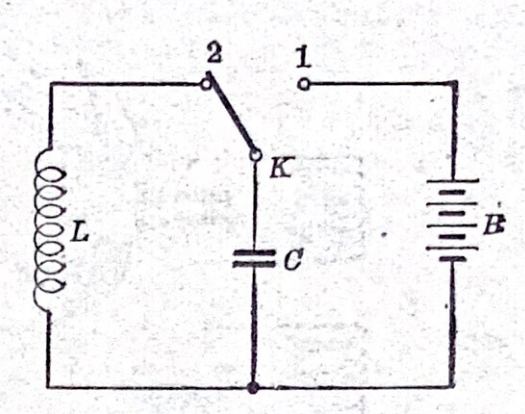
\includegraphics[width=0.5\linewidth]{lc-oscillation-circuit.png}
	\caption{LC 振荡电路示意图}
	\label{fig:oscillation-circuit}
\end{figure}

LC 振荡电路的工作过程可以分为多个阶段（如图\ref{fig:lc-oscillation-process}所示）：

\begin{enumerate}[leftmargin=0.5cm]
	\item \textbf{充电阶段}：将开关 K 拨到位置 1，使电容器 C 充电，此时电路中储存了一定的电场能。当充电结束而尚未放电的瞬时（图\ref{fig:lc-oscillation-process}(b)），电容器内的电场最强，电路中的能量全部为电场能。
	
	\item \textbf{放电阶段}：当开关拨到位置 2 后，电容器开始通过电感线圈放电。由于线圈的自感作用，电流不能立即达到最大值，而是逐渐增强，线圈周围的磁场也随之逐渐增强（图\ref{fig:lc-oscillation-process}(b)），同时电容器内的电场逐渐减弱，电场能逐渐转化为磁场能。当放电结束时（图\ref{fig:lc-oscillation-process}(c)），电场消失，磁场达到最大强度。
	
	\item \textbf{反向充电阶段}：此时电容器已完全放电，但电路中的电流并不会立即降为零。根据自感现象原理，线圈磁场的消失是一个逐渐减弱的过程，会产生与原电流方向相同的感应电流。这个感应电流使电容器两板重新带电，但电荷极性与原来相反（图\ref{fig:lc-oscillation-process}(d)），此过程称为反向充电，磁场能逐渐转化为电场能。
	
	\item \textbf{反向放电与循环阶段}：当磁场消失的瞬间，电容器完成反向充电。随后电容器又开始放电（图\ref{fig:lc-oscillation-process}(e)），产生与之前方向相反的电流；接着电容器再度充电（图\ref{fig:lc-oscillation-process}(f)）。如此周而复始，在振荡电路中就形成了周期性变化的振荡电流。
\end{enumerate}

\begin{figure}[H]
	\centering
	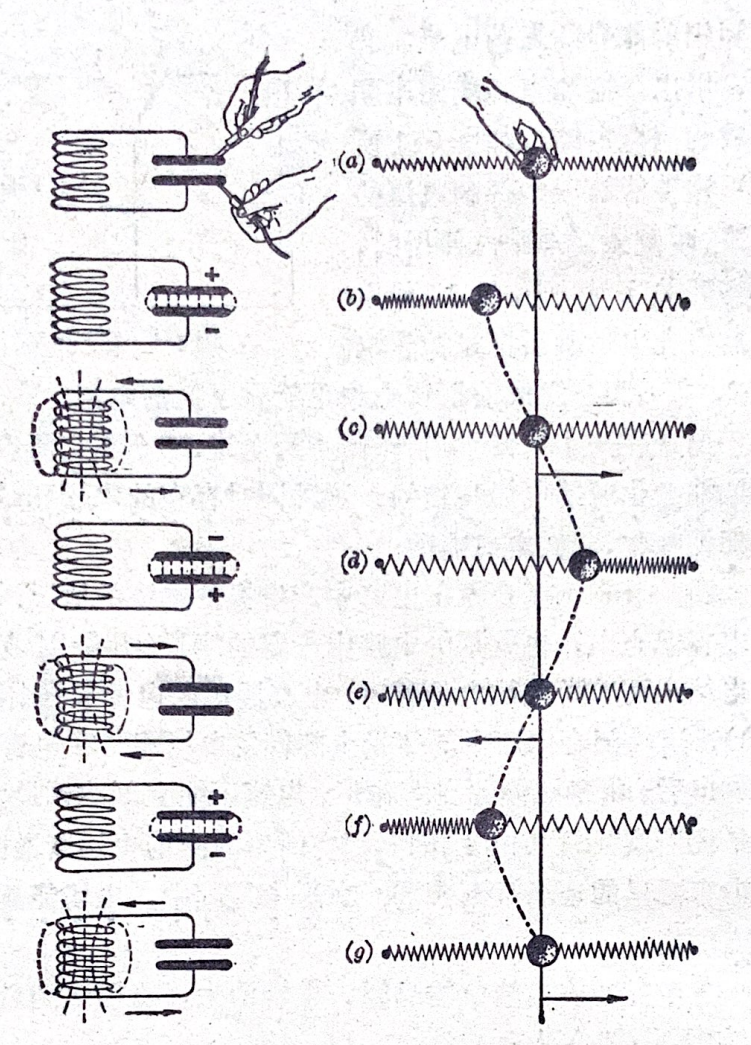
\includegraphics[width=0.8\linewidth]{lc-oscillation-process.png}
	\caption{LC 振荡电路工作过程示意图（a）充电完成；（b）开始放电；（c）放电完毕；（d）反向充电完成；（e）反向放电；（f）再度充电}
	\label{fig:lc-oscillation-process}
\end{figure}

如果在一个电路中有振荡着的电流，那么在它周围就会产生周期性变化的电场和磁场。这种同时存在的电场和磁场的周期性变化，就叫做电磁振荡。从能量转换的角度看，电磁振荡就是电场能与磁场能之间不断相互转换的过程。LC 振荡回路的固有频率由公式 $f = \frac{1}{2\pi\sqrt{LC}}$ 决定，通过选择合适的 L 和 C 值，可以获得从几百千赫兹到几百兆赫兹的高频振荡信号，这正是无线电通信所必需的载波频率范围。

电磁振荡与弹簧振子振动非常相似。在 LC 振荡电路中，电场能和磁场能的交替转变，类似于弹簧振子中弹性势能和动能的相互转换。当电容器充电完毕时，相当于弹簧振子被拉到最大位移处，此时电场能（类比势能）达到最大；当电容器放电完毕时，相当于弹簧振子通过平衡位置，此时磁场能（类比动能）达到最大。这种类比有助于我们理解电磁振荡的本质。

为了便于调整振荡频率，采用电感 $L$ 和电容 $C$ 组成的电路，振荡频率由电路本身的参数决定，这种振荡称为 \textbf{自由振荡}。在实际振荡过程中，由于电路中不可避免地存在电阻，会引起能量损失，导致振荡的振幅（电流强度的最大值）逐渐减小。振幅逐渐减小的振荡称为 \textbf{阻尼振荡} 或 \textbf{减幅振荡}，如图\ref{fig:damped-undamped-oscillation}(a)所示。

如果能在振荡过程中适时补充能量，以补偿电路的能量损耗，振荡的振幅就能维持不变。振幅不变的振荡称为 \textbf{无阻尼振荡} 或 \textbf{等幅振荡}，如图\ref{fig:damped-undamped-oscillation}(b)所示。

\begin{figure}[H]
	\centering
	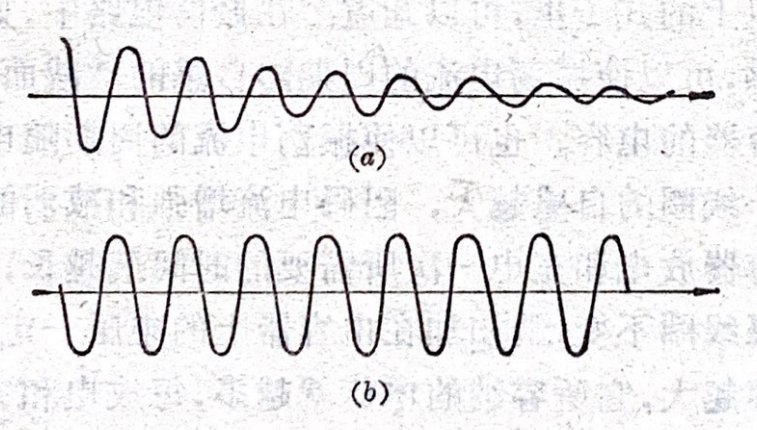
\includegraphics[width=0.8\linewidth]{damped-undamped-oscillation.png}
	\caption{阻尼振荡与无阻尼振荡波形图（a）阻尼振荡（减幅振荡）；（b）无阻尼振荡（等幅振荡）}
	\label{fig:damped-undamped-oscillation}
\end{figure}

在无线电技术中，需要使用等幅振荡来产生稳定的高频载波信号。

\subsection{振荡电流的周期和频率}

在振荡电路中，通过某一点的电流，由某个方向的最大值再恢复到这个方向的最大值时，我们就说电流完成了一次全振荡。完成一次全振荡所经过的时间，叫做振荡电流的 \textbf{周期}（用 $T$ 表示），单位为 \textbf{秒（s）}；在 1 秒钟内完成全振荡的次数，叫做振荡电流的 \textbf{频率}（用 $f$ 表示），单位为 \textbf{赫兹（Hz）}。周期和频率的关系为：

\[ f = \frac{1}{T} \]

常用的频率单位还有千赫（kHz，$10^3$ Hz）和兆赫（MHz，$10^6$ Hz）。例如，中波广播的频率范围约为 531 kHz 至 1602 kHz，调频广播的频率范围约为 87.5 MHz 至 108 MHz。

在无阻尼振荡电路中，振荡周期由电路本身的性质决定，我们把这个周期叫做振荡电路的 \textbf{固有周期}，相应的振荡频率叫做 \textbf{固有频率}。对于 LC 振荡电路，其固有周期和固有频率由电感 $L$ 和电容 $C$ 的值决定：

\[ T = 2\pi\sqrt{LC} \]
\[ f = \frac{1}{2\pi\sqrt{LC}} \]

其中，电感 $L$ 的单位为 \textbf{亨利（H）}，电容 $C$ 的单位为 \textbf{法拉（F）}。在实际应用中，电感常用毫亨（mH，$10^{-3}$ H）或微亨（μH，$10^{-6}$ H）作为单位，电容常用微法（μF，$10^{-6}$ F）或皮法（pF，$10^{-12}$ F）作为单位。

由此可见，振荡电路的周期（或频率）与电感和电容的关系如下：

\begin{itemize}[leftmargin=1cm]
	\item 如果增大线圈的自感，振荡电流的周期会随之增大（频率减小）；反之，减小自感，周期会减小（频率增大）。这是因为线圈的自感越大，阻碍电流变化的作用越强，电容器充放电一次所需的时间就越长。
	\item 如果增大电容器的电容，振荡电流的周期也会随之增大（频率减小）；反之，减小电容，周期会减小（频率增大）。这是因为电容越大，在相同电压下容纳的电荷越多，充放电一次所需的时间就越长。
\end{itemize}

由此可见，我们可以通过两种方法来改变振荡电路的周期（或频率）：
\begin{enumerate}[leftmargin=1cm]
	\item \textbf{改变线圈匝数}：增加线圈匝数会增大自感，减少匝数则减小自感；
	\item \textbf{使用可变电容器}：通过改变极板间距或重叠面积来调整电容。
\end{enumerate}

在无线电技术中，这两种方法都被广泛采用。例如，收音机的调谐电路通常同时使用可变电容和带有磁芯的线圈，通过调整电容来进行粗调，通过移动磁芯来进行微调，从而精确选择所需的电台频率。

\section{电磁波和电磁波的发送}

振荡电路里产生振荡电流的时候，在它周围空间会产生不可分割的电场和磁场。电磁场理论指出：任何电场的变化都会在它周围空间产生变化的磁场，任何磁场的变化都会在它周围空间产生变化的电场。由此可见，电场和磁场有着极为密切的关系，电场和磁场原来是一种统一的客观物质——\textbf{电磁场}——的两个方面。

如果在空间某处有一根导线（如图\ref{fig:electromagnetic-wave-generation}所示），当导线中有振荡电流时，它的周围就会产生变化的磁场；变化的磁场在附近空间又会产生变化的电场；这种变化的电场又会产生新的变化的磁场。这种不断交替变化的电场和磁场，会越来越远地向周围空间传播，就形成了\textbf{电磁波}。因此，电磁波就是在空间传播的电磁场。

\begin{figure}[H]
	\centering
	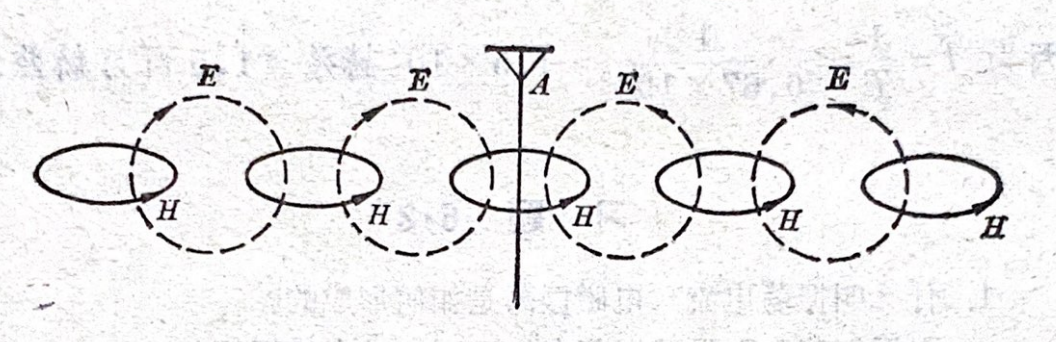
\includegraphics[width=0.8\linewidth]{electromagnetic-wave-generation.png}
	\caption{电磁波产生示意图}
	\label{fig:electromagnetic-wave-generation}
\end{figure}

实验和理论都表明，电磁波的传播速度非常大，在真空中它等于光的速度，约为 $c \approx 3 \times 10^8$ 米/秒（即 $3 \times 10^{10}$ 厘米/秒）。在空气中，电磁波的传播速度非常接近这一数值。

在电磁波的传播过程中，电场强度和磁场强度彼此之间永远互相垂直，并且它们都垂直于电磁波的传播方向。因此，电磁波是一种\textbf{横波}，如图\ref{fig:electromagnetic-wave-propagation}所示。

\begin{figure}[H]
	\centering
	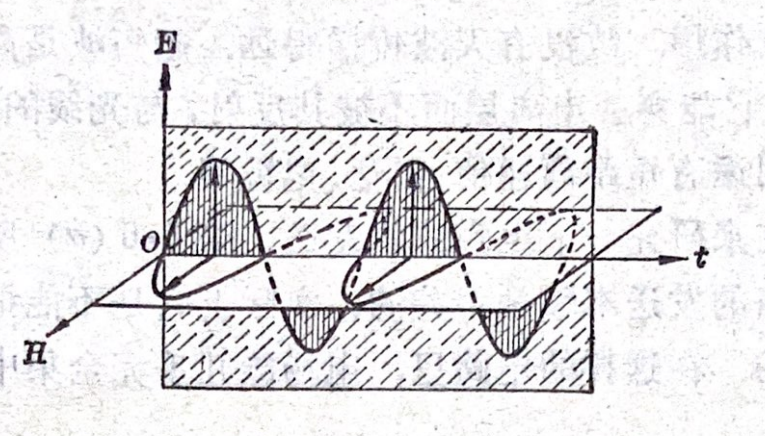
\includegraphics[width=0.8\linewidth]{electromagnetic-wave-propagation.png}
	\caption{电磁波传播示意图}
	\label{fig:electromagnetic-wave-propagation}
\end{figure}

\subsection{电磁波的发送}

现在来研究一下电磁波的发送。如图\ref{fig:oscillation-circuit-evolution}(a)所示的闭合振荡电路，其辐射电磁波的能力是很差的，实际上几乎不能把电磁波发送出去。在这种电路里，电场能几乎完全集中在电容器的两块极板之间，磁场能几乎完全集中在电感线圈内部，辐射出去的能量极少。我们把这种振荡电路叫做\textbf{闭合振荡电路}。

如果把电路改成如图\ref{fig:oscillation-circuit-evolution}(b)所示的形式，即将电容器的极板拉开，它的辐射本领会有所改善；但如果改成如图\ref{fig:oscillation-circuit-evolution}(c)所示的形式，将电容器的一个极板去掉，另一个极板变成天线，线圈也部分开放，它的辐射本领就更好了。在无线电技术中，经常使用图(c)所示的电路，我们称它为\textbf{开放振荡电路}。

\begin{figure}[H]
	\centering
	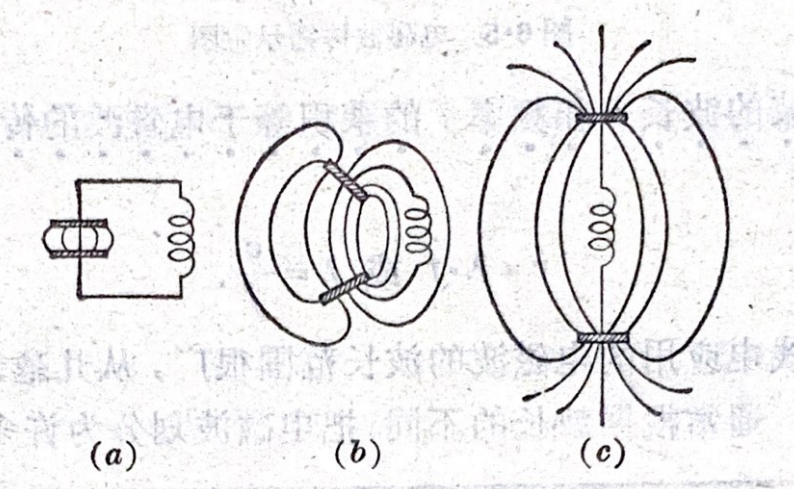
\includegraphics[width=0.8\linewidth]{oscillation-circuit-evolution.png}
	\caption{振荡电路的演变（a）闭合振荡电路；（b）半开放振荡电路；（c）开放振荡电路（天线）}
	\label{fig:oscillation-circuit-evolution}
\end{figure}

开放振荡电路之所以能有效辐射电磁波，是因为它将电场和磁场的能量分散到更大的空间范围，使得振荡电流产生的变化电场和变化磁场能够更有效地相互激发并向外传播，从而形成电磁波。

在实际应用中，通常采用\textbf{感应耦合}的方式来激发开放振荡电路。如图\ref{fig:inductive-coupling}所示，一个开放振荡电路（AL₁B）和一个闭合振荡电路（CL₂）通过互感线圈L₁和L₂相耦合。当闭合电路中产生振荡电流时，由于L₁和L₂之间的互感作用，会在开放电路中感应出相同频率的振荡电流。

开放电路中伸向空中的导线A叫做\textbf{天线}，与地面相连的导线B叫做\textbf{地线}。电磁波就是通过天线和地线组成的开放电路发送出去的。这种通过互感耦合实现电磁波发送的方法，是无线电通信中常用的技术。

\begin{figure}[H]
	\centering
	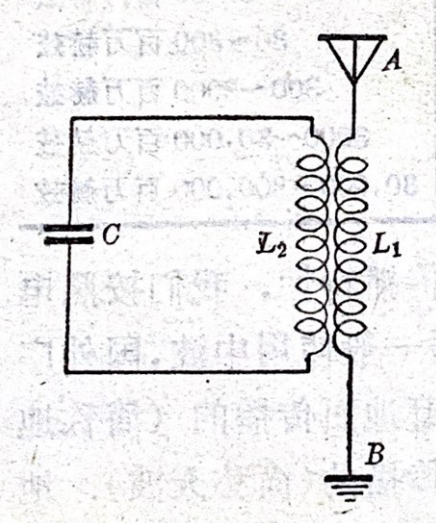
\includegraphics[width=0.8\linewidth]{inductive-coupling.png}
	\caption{感应耦合发送电路示意图（AL₁B为开放振荡电路，CL₂为闭合振荡电路）}
	\label{fig:inductive-coupling}
\end{figure}

\subsection{电磁波的波长}

什么是电磁波的波长呢？与机械波相似，在振荡电流完成一次全振荡的时间（即周期 $T$）内，电磁场在空间传播的距离，就是电磁波的\textbf{波长}（用 $\lambda$ 表示）。

电磁波的波长 $\lambda$、频率 $f$ 和传播速度 $c$ 之间存在如下关系：

\[ c = \lambda f \]

由此可推导出：

\[ \lambda = \frac{c}{f} \]

这表明，电磁波的波长与频率成反比。频率越高，波长越短；频率越低，波长越长。

无线电应用的电磁波波长范围很广，从几毫米到 3000 米以上。通常根据波长的不同，将电磁波划分为多个波段。各波段的波长和频率范围如下表所示：

\begin{table}[H]
	\centering
	\begin{tabular}{|l|l|l|}
		\hline
		\textbf{名称} & \textbf{波长} & \textbf{频率} \\
		\hline
		长波 & 3000 米以上 & 低于 100 kHz \\
		\hline
		中波 & 200～3000 米 & 100～1500 kHz \\
		\hline
		中短波 & 50～200 米 & 1500～6000 kHz \\
		\hline
		短波 & 10～50 米 & 6～30 MHz \\
		\hline
		超短波（米波） & 1～10 米 & 30～300 MHz \\
		\hline
		分米波 & 0.1～1 米 & 300～3000 MHz \\
		\hline
		厘米波 & 0.01～0.1 米 & 3000～30000 MHz \\
		\hline
		毫米波 & 0.001～0.01 米 & 30000～300000 MHz \\
		\hline
	\end{tabular}
	\caption{无线电电磁波各波段划分}
	\label{tab:radio-wave-bands}
\end{table}

不同波段的无线电波具有不同的传播特性，我们可以根据实际需求选择合适的波段。例如，长波主要用于远距离通信和导航，中波用于国内调幅广播，短波用于国际广播和通信，超短波用于调频广播和电视信号传输，而微波（分米波、厘米波、毫米波）则广泛应用于雷达、卫星通信和微波炉等领域。

中波主要沿着地面传播（简称\textbf{地波}），而短波主要依靠电离层的反射传播（简称\textbf{天波}）。地波传播的信号比天波更稳定，通信更可靠，但由于地面的吸收作用，地波的传播距离不如天波远。天波通过电离层的反射可以实现远距离甚至跨洲际通信，但受季节、昼夜和太阳活动等因素的影响较大。

超短波是高频率的无线电波，它能够穿透电离层而不被反射，传播特性与光线相似，主要进行直线传播，因此适用于短距离通信、雷达和电视信号传输等。

\subsection{广播常用波段}

波段指的是无线电波中一段特定的频率范围。日常收听的广播主要涉及以下几个频段：

\textbf{长波 LW 波段：}广播用频率主要在 153–279 kHz。采用 AM 调制方式。传播方式以地波为主，信号沿地表可稳定传输数百甚至上千公里，受昼夜和电离层扰动的影响很小，信号稳定可靠。但由于波长极长（约 1000–2000 米），天线尺寸大、发射设备成本高，且频带窄（仅约 126 kHz）、音质不及调频广播。目前仅有欧洲、北非、蒙古及俄罗斯部分地区保留了长波广播电台（如法国 Intercontinental、英国 BBC Radio 4、罗马尼亚 Radio Romania Actualitati 等），主要用于广袤偏远地区的基础覆盖、导航授时以及对潜艇通信等特殊用途。中国内地没有民用长波广播频率分配。

\textbf{中波 MW 波段：}主流范围：525–1605 kHz（中国/欧洲），北美地区扩展至 535–1705 kHz。中国实际使用标准为 531–1602 kHz，采用 9 kHz 频道间隔。采用 AM 调制方式。电波可经地波和天波两种方式传播：白天主要依靠地波，覆盖半径约几十到上百公里；夜间电离层 D 层消失，电波能通过 F 层反射实现远距离接收，覆盖范围可达数百甚至上千公里，远超调频广播。中波广播信号稳定，是城市和农村地区最主要的广播覆盖手段之一。

\textbf{短波 SW 波段：}主流广播范围通常为 2.3–26.1 MHz（2300–26100 kHz），国际电联将其划分为多个米波段便于识别（如 49 米波段 5900–6200 kHz、41 米波段 7200–7450 kHz、31 米波段 9400–9900 kHz、25 米波段 11600–12100 kHz、19 米波段 15100–15800 kHz、16 米波段 17480–18030 kHz、13 米波段 21450–21950 kHz 等）。采用 AM 调制方式，部分采用 SSB（单边带）调制。属于高频频段，电波主要通过天波传播——向天空发射后被电离层反射回地面，反射后可再次跳跃，从而实现数百至数千公里甚至跨洲际的远距离接收。短波信号受季节、昼夜、太阳活动周期及电离层变化影响很大，不同时间宜选用不同频段；音质通常不及调频广播，且存在衰落现象，但仍是国际广播、业余无线电与应急通信的重要媒介。

\textbf{超短波 FM 波段：}主流范围 87.5–108 MHz（中国/欧洲），频道间隔 0.1 MHz。其中 87.5–88.0 MHz 主要用于校园广播和教学电台，88.0–108.0 MHz 用于公共广播。属于甚高频（VHF）频段，电波近似直线传播，绕射能力弱，覆盖范围通常限于视距（约 30–50 公里），但音质优良（可传输立体声）、抗干扰能力强，是城市地区最受欢迎的广播方式。

\section{调制}

无线电发送机发出的电磁波需要能够传递某种信号。例如，在无线电报中，电磁波必须随电码符号而改变；在无线电广播中，电磁波必须随声音而改变；在电视广播中，电磁波必须随图像而改变。因此，在无线电发送机中，必须先将电码、语言、音乐等信号转换为低频电压信号，再将低频电压信号加载到高频电磁波上发送出去。这种把低频信号加在高频电磁波上的过程，就叫做\textbf{调制}。

在调制过程中，涉及几个重要概念：
\begin{itemize}[leftmargin=1cm]
	\item \textbf{调制信号}：需要发送的原始信号，如声音、图像、电码等；
	\item \textbf{载波}：未调制的高频电磁波，作为信号的"运输工具"；
	\item \textbf{调制波}：载有低频信号的高频电磁波。
\end{itemize}

举一个通俗的例子：高频电磁波就像是一列火车（载波），低频信号就像是货物（调制信号），而调制就是将货物装上火车的过程，最终形成载有货物的火车（调制波）。

收音机是将调制过的音频信号解调、放大，最后通过扬声器等输出的设备。那么为什么不能直接接收未调制的音频信号呢？

音频信号的频率范围通常在 20 Hz 到 20 kHz 之间，属于低频信号。这样的低频信号如果直接通过天线发射，会遇到两个主要问题：

\begin{enumerate}[leftmargin=1cm]
	\item \textbf{天线效率极低}：天线的有效长度通常需要与信号波长的四分之一相当。对于 1 kHz 的音频信号，根据波长公式 $\lambda = c / f$，其中光速 $c \approx 3 \times 10^8$ m/s，可算出波长约为 300 公里，所需天线尺寸巨大，无法实际实现。
	\item \textbf{信道复用困难}：可用的音频频段非常窄，且拥挤不堪。如果不经调制直接发射，所有电台的信号都会混在一起，互相干扰，因为所有音频信号都挤在同一频段，接收端无法通过调谐来分离不同电台。
\end{enumerate}

收音机接收到的电台信号通常有两种，调幅 AM 和调频 FM。波形图如下：

\begin{figure}[H]
	\centering
	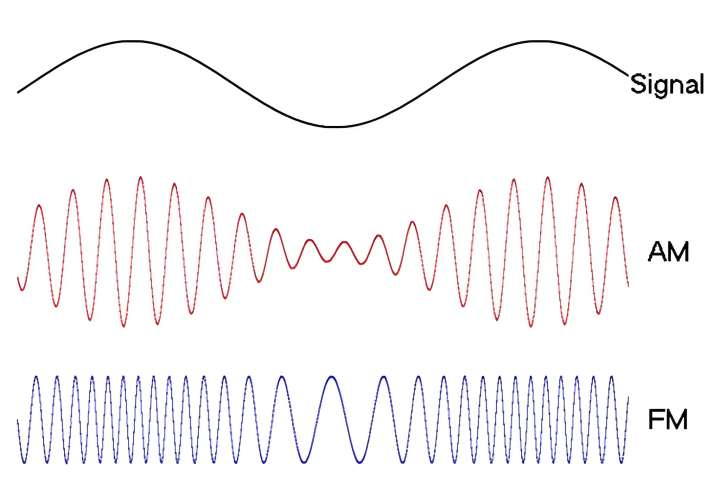
\includegraphics[width=0.7\linewidth]{am-fm-waveform.jpg}
	\caption{AM 与 FM 波形图}
	\label{fig:am-fm}
\end{figure}

从上图可以看出来：

\begin{itemize}[leftmargin=1cm]
	\item AM：载波的振幅随音频信号变化，但频率不变。
	\item FM：载波的频率随音频信号变化，但振幅不变。
\end{itemize}

实际上，任何一个载波都有三个基本参数：振幅、频率和相位。调制过程本质上就是使载波的某一个或多个参数随着调制信号而变化。根据改变的参数不同，对应的调制方法可以分为：

\begin{itemize}[leftmargin=1cm]
	\item \textbf{调幅（AM）}：改变载波的振幅；
	\item \textbf{调频（FM）}：改变载波的频率；
	\item \textbf{调相（PM）}：改变载波的相位。
\end{itemize}

以上过程称为调制，解调是其相反过程，会在后面进行说明。

\subsection{调幅的工作原理}

调幅是使载波的振幅随着低频信号的波形而变化的调制方式。在无线电广播中，调制器通常利用话筒或拾音器来完成。下面介绍调幅的简单原理：

如图\ref{fig:carbon-microphone-modulator}所示，M是一只炭精话筒，将它串联在天线和地线的开放电路中。

\begin{figure}[H]
	\centering
	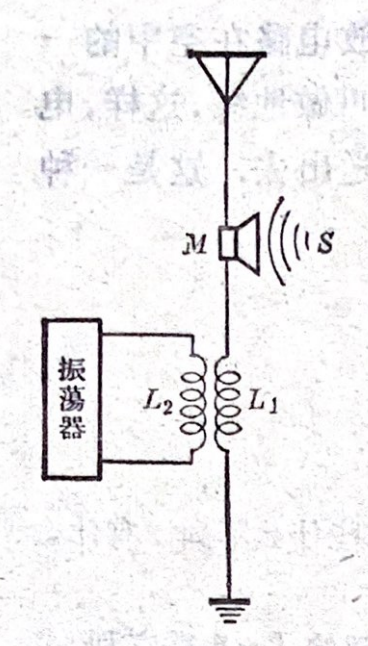
\includegraphics[width=0.7\linewidth]{carbon-microphone-modulator.png}
	\caption{炭精话筒调制器示意图}
	\label{fig:carbon-microphone-modulator}
\end{figure}

当没有向话筒说话时，话筒上的金属薄片不振动，话筒里炭粒的松紧程度不变化，因此话筒的电阻也无变化。这时，发送天线电路里的高频振荡电流的振幅是均匀的，如图\ref{fig:oscillation-current-amplitude}所示。

\begin{figure}[H]
	\centering
	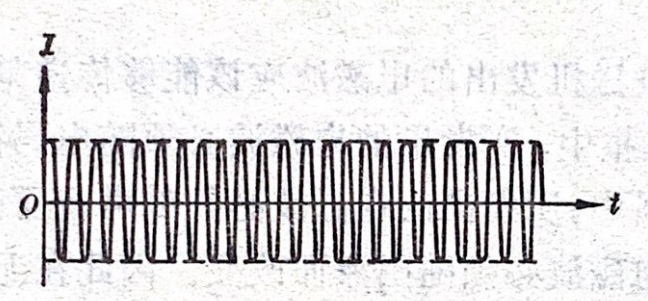
\includegraphics[width=0.8\linewidth]{oscillation-current.png}
	\caption{天线电路里的振荡电流（未调制）}
	\label{fig:oscillation-current-amplitude}
\end{figure}

当对话筒说话时，话筒上的金属薄片随着声波而振动，炭粒的松紧程度随着金属片的振动而改变，因此话筒的电阻也随着声音振动而增减。这时，天线电路里的交变电动势虽然是等幅的，但由于电阻值时大时小，振荡电流的强度就相应地跟着时小时大，因此发送出去的电磁波的振幅也就不均匀了。如图\ref{fig:oscillation-current-modulated}所示。

\begin{figure}[H]
	\centering
	
\includegraphics[width=0.8\linewidth]{am_modulation.jpg}
	\caption{天线电路里的振荡电流（调幅后）}
	\label{fig:oscillation-current-modulated}
\end{figure}

振幅的改变是随着声音振动而变化的。这种依照声音振动而改变振幅的电磁波叫做\textbf{调幅波}。调幅广播就是利用调幅波来传递声音信号的。

\subsection{调频的工作原理}

调频就是使载波的频率随着低频信号的频率而变化的调制方式。当载波被低频调制信号调制后，形成了调频信号波。

在调频波的频率变化中，不但反映了调制信号电压正负的变化，也反映了调制信号电压振幅的变化。调频波是等幅波，不管频率发生怎样的偏移，它的振幅都不改变。调频波抵抗干扰的能力比较强，在传递过程中失真比较小，因此在现代通信中应用广泛，如调频广播、电视伴音和数据传输等。

\subsection{调相的工作原理}

调相就是使载波的相位随着音频信号的相位而变化的调制方式。与调幅和调频相比，调相在模拟通信中的应用相对较少，但在数字通信中（如相移键控 PSK）有广泛应用。调相波同样具有抗干扰能力强的特点，但解调电路相对复杂。

\section{电谐振}

当我们要收听无线电广播时，会习惯地把收音机上的旋钮拧到不同的位置，用它来寻找要听的电台，这究竟是根据什么道理呢？

世界各国有无数的无线电发送电台，它们发出各种不同频率的电磁波。这些电磁波在空间传播遇到接收天线时，在天线电路里就会依照原有的频率产生感生电流。如果我们不经选择地把它们都接收下来，并都变成声音信号，那将除了一片嘈杂声音外，什么也分辨不出。因此我们必须设法在这些感生电流中选择出所需要的频率，并且把接收到的电磁波设法形成相当强的振荡电流，其他不需要的，就让它尽量地微弱。

这种从众多频率中选择特定频率的现象叫做\textbf{电谐振}，也称为\textbf{调谐}。通过调节收音机中的可变电容器或电感线圈，可以改变接收电路的固有频率，使其与我们想要接收的电台频率一致，从而发生谐振，选出该电台的信号。

学习单摆振动时，我们知道当A摆的摆长等于B摆的摆长时，策动力变化的频率就等于B摆的固有频率，这时就发生共振。发生共振时物体作受迫振动的振幅是最大的。

电磁振荡也是如此，当振荡电路的固有频率跟接收来的电磁波的频率（或加在电路上的交变电压的频率）相同时，电路里激起的感生电流就最强，在电学中，这种现象叫做电谐振现象。

电谐振的条件是两个振荡电路的固有频率相同。设发送电路的固有频率为 $f_1$，接收电路的固有频率为 $f_2$，则：

\[
f_1 = \frac{1}{2\pi\sqrt{L_1C_1}}, \quad f_2 = \frac{1}{2\pi\sqrt{L_2C_2}}
\]

只有在 $f_1 = f_2$，即 $L_1 \cdot C_1 = L_2 \cdot C_2$ 时才会发生电谐振。

如图\ref{fig:radio-tuning-circuit}所示，在天线线圈旁边耦合一个带有可变电容器的振荡电路，这样就构成了选择电台的装置。把旋钮拧到不同位置，实质上是用调节电容（或调节电感）的方法使闭合电路的固有频率和我们所要接收的频率相同。这时如果天线电路里有这种频率的振荡电流存在，也就是如果空间里有这种频率的电磁波存在，就会对闭合电路起感应作用，形成电谐振现象，那么这个电磁波在电路中激起的振荡电流比其他频率的振荡电流强得多，这样就收到我们所需要的电磁波。

\begin{figure}[H]
	\centering
	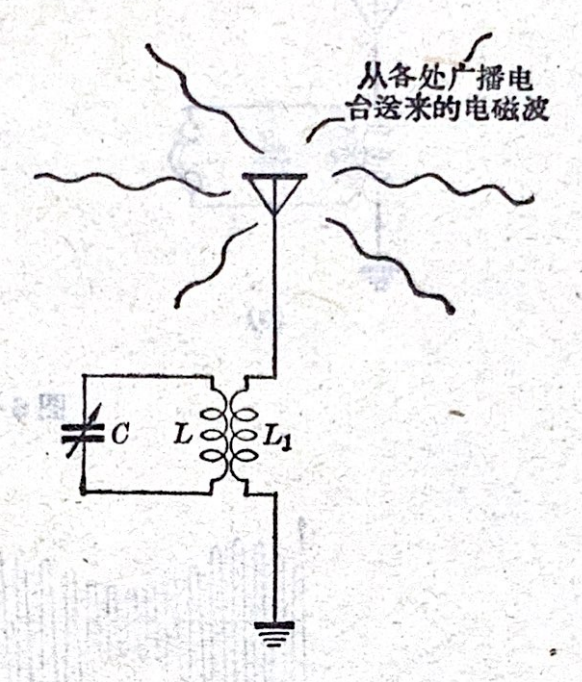
\includegraphics[width=0.8\linewidth]{radio-tuning-circuit.png}
	\caption{LC调谐电路示意图（C为可变电容器，L为电感线圈，L₁为天线耦合线圈）}
	\label{fig:radio-tuning-circuit}
\end{figure}

用这样的方法选择电磁波，叫做调谐。在无线电技术中，是利用LC调谐电路的谐振作用来完成这一任务的。

明确了什么是调制以及电台信号所在的波段后，接下来我们看看收音机内部是如何将电波还原成声音的。

\part{矿石收音机}
\label{part:crystal-radio}

\chapter{矿石收音机基础}
\label{chap:crystal-radio-basics}

\section{无线电发明者：亚历山大·斯捷潘诺维奇·波波夫}

在正式介绍矿石收音机之前，有必要了解无线电技术发展史上的重要人物——俄国科学家亚历山大·斯捷潘诺维奇·波波夫（Александр Степанович Попов，1859–1906）。

波波夫于1859年出生于乌拉尔山区的一个牧师家庭，自幼热爱科学，尤其对电磁学表现出浓厚兴趣。1882年毕业于圣彼得堡大学物理数学系后，进入喀琅施塔得海军军官学校担任物理学教员。在此期间，他密切关注德国物理学家海因里希·赫兹（Heinrich Hertz）关于电磁波的实验研究，并致力于将电磁波理论应用于实际通信。

1895年5月7日，波波夫在俄罗斯物理化学学会年会上公开演示了他研制的雷电指示器——这是世界上首台带有天线的无线电接收装置。该装置能够检测远距离雷电产生的电磁波信号。1896年3月24日，波波夫成功实现了约250米距离内的无线报文传输，发送的内容为"Heinrich Hertz"，以纪念这位电磁波发现者。这标志着无线电从实验室走向实际应用的重要一步。

值得注意的是，与波波夫同一时期，意大利工程师古列尔莫·马可尼（Guglielmo Marconi）也在独立进行无线电报的研究工作。两人几乎同时在1890年代中期取得了突破性进展，因此关于"无线电之父"的归属问题，学术界至今仍存在不同观点：西方国家普遍推崇马可尼的贡献，而俄罗斯及东欧国家则强调波波夫的开创性地位。客观而言，两人的工作都是独立完成的，都对无线电技术的发展做出了不可磨灭的贡献。

然而在当时，沙皇政府对波波夫的发明并未给予足够重视。尽管波波夫已在海军中成功应用了无线电通信系统，沙皇政府仍然倾向于向国外购买海军舰艇所用的无线电报设备，这种状况直到1917年十月革命后才得到根本改变。苏联政府高度重视波波夫的历史贡献，不仅将其尊为"无线电之父"，还设立了以他名字命名的各种奖章和奖项，用以表彰那些为祖国无线电事业发展做出突出贡献的科技工作者。每年的5月7日也被定为"无线电节"，以纪念这一具有里程碑意义的日子。

\section{检波}

为了实现无线电通信或广播，必须把要传送的低频信号加到高频电磁波上传送出去，也就是用低频信号对高频电磁波进行调制。当收音机收到已调制的高频电磁波后，必须把接收机的谐振电路调到和这个已调幅波发生谐振（对其他电台发送的已调幅波不起谐振），这样，需要接收的电台所发送的已调幅波就被接收下来。但实验证明，把听筒直接接在电路上，如图\ref{fig:detector-circuit}(a)所示，是听不到声音的。

\begin{figure}[H]
	\centering
	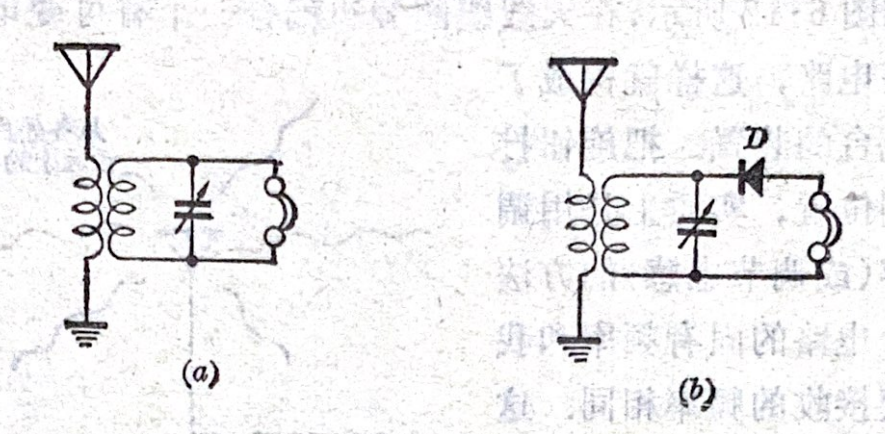
\includegraphics[width=0.8\linewidth]{detector-circuit.png}
	\caption{检波电路示意图（a）直接接听筒；（b）带有检波器的电路}
	\label{fig:detector-circuit}
\end{figure}

为什么听不到声音呢？

假设调谐回路收到一个由简单的正弦低频信号调幅的高频电磁波，那么，在听筒中流过的电流也是形状完全相同的高频振荡电流。获得了高频振荡电流还不等于收到了随电磁波带来的声音。

我们知道，听筒是依靠电磁铁在起作用的，电磁铁线圈的自感系数很大，高频振荡电流是不容易通过的。同时听筒中成声铁片的固有频率很低。当高频电流的正半周要使听筒的铁片向一方振动时，紧接着它的负半周就要使铁片向另一方振动（高频电流的频率是很高的，例如在中波波段，是从 531 kHz 到 1602 kHz）。由于铁片的机械惯性与这样快的振动不相适应（还没有开始向一方振动时，电流就又已经改变了方向），因此，它的振动非常微弱，以至根本听不到声音。

这是因为高频振荡电流变化太快，无法使听筒的振动膜振动。因此，我们需要从接收到的高频调幅波中取出低频音频信号，这个过程叫做\textbf{检波}，也称为\textbf{解调}。检波是调制的逆过程，它能将音频信号从高频载波中分离出来，使听筒能够还原出声音。

\begin{figure}[H]
	\centering
	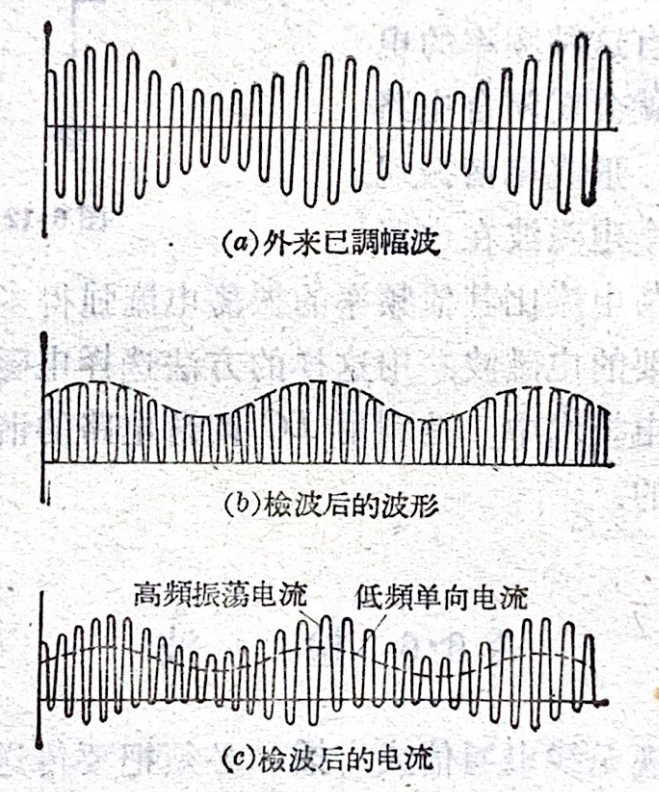
\includegraphics[width=0.8\linewidth]{detector-waveforms.png}
	\caption{检波过程波形图（上图：调幅波波形；中图：检波后波形；下图：检波后的电流）}
	\label{fig:detector-waveforms}
\end{figure}

在收音机中，检波是利用具有\textbf{单向导电性}的装置来完成的，如半导体二极管或电子管，这种装置叫做\textbf{检波器}。矿石收音机中使用的矿石（如方铅矿、黄铁矿）就是一种天然的半导体检波器。

\section{矿石收音机总述}

这是最经典的入门电路，借用前辈书中的插图，最简单的电路和接线图如下：

\begin{figure}[H]
	\centering
	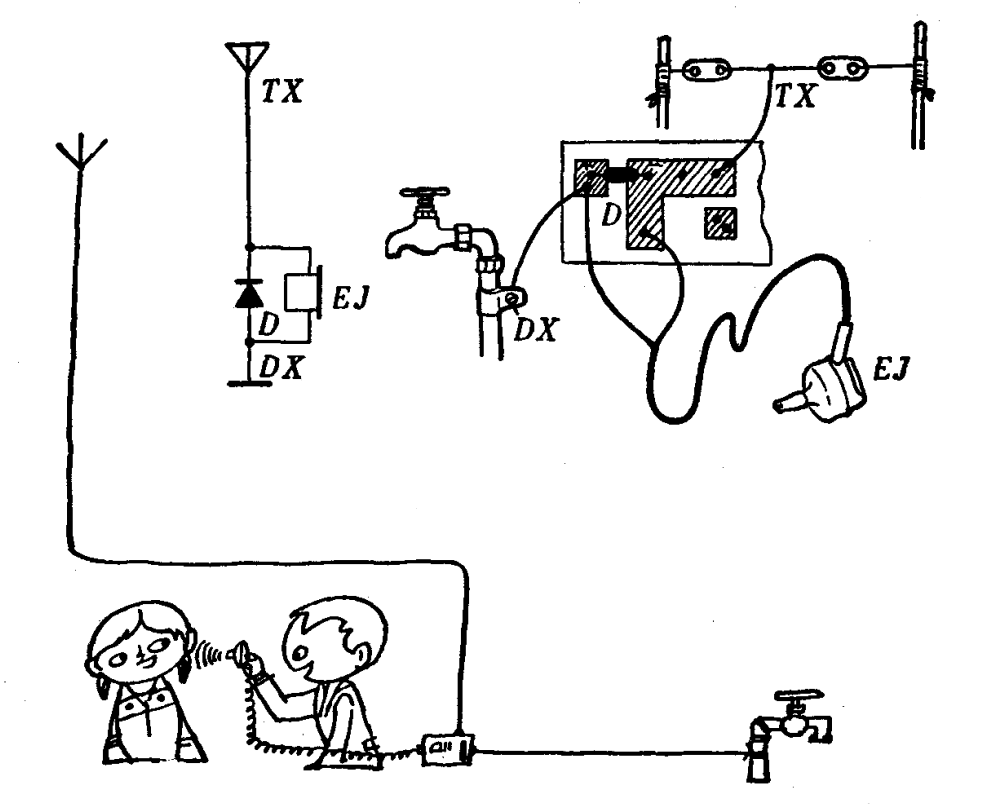
\includegraphics[width=0.7\linewidth]{simple_radio_circuit.png}
	\caption{矿石收音机电路图。图片来源：朱蔼初编著的《看图学装收音机》}
	\label{fig:crystal-radio-circuit}
\end{figure}

图中展示的是矿石收音机的典型结构，它由天线、晶体二极管、耳机、地线 4 个核心部件组成，本质上是一个无源接收装置。它利用半导体材料的整流特性接收无线电信号，不需要外接电源，完全依靠天线接收的无线电波能量工作。适用于接收 AM 电台的信号。

\section{各部件功能}

\subsection{天线}

接收空间中传播的无线电波，这些电波会在天线中感应出微弱的高频交变电流。

在两个绝缘的竿子之间横拉一根电线即可，高度越高越好。在楼上，可用鱼竿挑出一根电线，离开墙体越远越好，谨防掉落。

\textbf{特别警示}：架设天线必须高度重视防雷，雷雨天气严禁使用，并应采取必要的避雷措施！

\subsection{二极管}

作为检波器，利用半导体的"单向导电性"，对天线接收到的高频信号进行检波（将调幅信号的高频载波去掉，提取音频信号）。

早期使用矿石检波器，这就是矿石收音机中"矿石"二字的来源。有活动矿石和固定矿石两种。活动矿石和固定矿石结构类似，核心就是矿石。常见有黄铁矿、方铅矿、红锌矿、自然铜等的金属矿石，结构如图。

\begin{figure}[H]
	\centering
	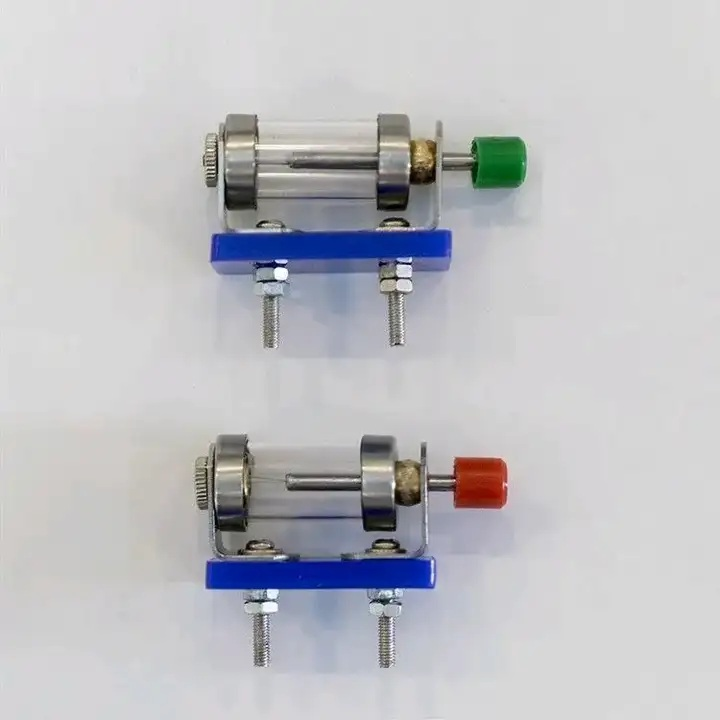
\includegraphics[width=0.7\linewidth]{mineral-detector.jpg}
	\caption{矿石检波器}
	\label{fig:mineral-detector}
\end{figure}

现在已无此必要，因为矿石价格不菲、调整麻烦且效果不理想。建议采用晶体二极管替代。型号可选 2AP9、1N60P 等，根据经验，1N60P 是个不错的选择。

\begin{figure}[H]
	\centering
	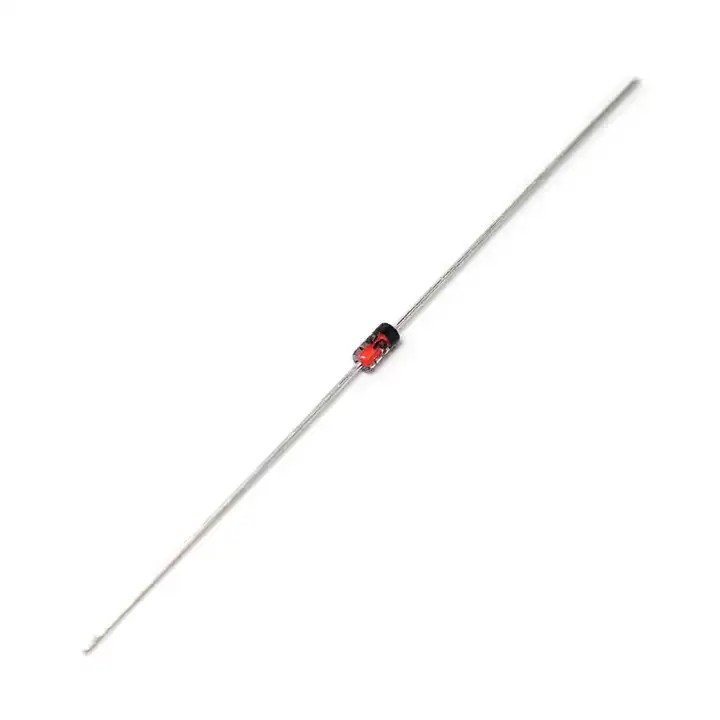
\includegraphics[width=0.7\linewidth]{1n60p.jpg}
	\caption{1N60P 二极管}
	\label{fig:1n60p}
\end{figure}

如果纯粹出于怀旧，完全可以采用矿石检波器，采购成品或自制皆可。

\textbf{注}：有资料称部分 1N60P 不适用，但笔者暂未遇到，待有机会再补充。

\subsection{耳机}

将晶体二极管输出的微弱音频信号转化为声波，供人耳收听。

此处必须使用高阻耳机，但目前市面上能买到的普通高阻耳机，其阻抗往往仍不满足矿石机的要求。

淘宝上能买到专为矿石机和电台设计的高阻耳机，但多为库存老货，可用，但价格较高。

更经济的替代方案是，使用阻抗匹配变压器加上普通低阻耳机（如手机耳机）的组合。

\subsection{地线}

连接到大地，相为天线感应到的电流提供一个完整的回路参考点，同时还能过滤掉一部分杂波干扰。

在农村的话，插根钢筋到地里就行，如自来水管是金属管的话，接在上面也可以。如果在楼房里，卫生间的等电位端子排是个不错的选择。\textbf{绝对禁止使用燃气管作为地线，有爆炸风险！}

\section{工作原理}

当电台发出的无线电波经过天线时，会在天、地线之间感应出一个高频信号电压来。如果仅接有一个耳机时，由于信号频率大大地高出音频范围，因此听不到声音。

在接上二极管后，高频电流从地线流向天线时，二极管正向导通，电流从二极管这一边流过，耳机被"旁路"；高频电流从天线流向地线时，二极管反向截止，电流只能被迫从耳机这一边的电路里流过。这就相当于一个开关，只让单向的电流脉冲流过耳机。

这个方向不变、强度随时间变化的脉动高频电流，其包络线形状和音频信号完全一致，音频信号就这样被"剥离"了下来。

最后，当这个携带音频信号的单向脉动电流流过耳机时，耳机线圈具有一定的电感特性，对高频成分阻抗很大，高频电流难以通过，相当于被"过滤"掉了；而低频的音频电流则可以顺利通过，驱动耳机振膜，最终发出人耳能听到的声音。

\section{总结}

这套装置极其简单，成本最低，且完全无需电源，这是它最大的魅力所在。

但它也有两个源于原理的明显缺点：

\begin{enumerate}[leftmargin=2cm]
	\item \textbf{选择性差}：无法筛选特定频率的电台，会同时收到多个频率的广播信号，导致声音混杂。
	\item \textbf{灵敏度低}：天线接收的能量很微弱，检波后的电流驱动耳机的功率有限，只能听到附近强功率电台的声音，而且音量很小。
\end{enumerate}

为了克服这些缺点，后来经典的矿石收音机会加入由可变电容和电感组成的谐振回路，通过调节电容来改变谐振频率，从而选择想要收听的电台，这也就是收音机调谐旋钮的前身。


\chapter{调谐电路}
\label{chap:tuning-circuit}

\section{带调谐电路的矿石收音机}

前面讲的收音机有个主要的问题，即无法筛选特定频率的电波，会同时收到多个广播信号，声音混杂在一起，影响收听。

为了解决这个问题，可在其基础上增加调谐电路。整机电路图如下：

\begin{figure}[H]
	\centering
	%\includegraphics[width=0.7\linewidth]{Images/}
	\caption{带调谐电路的矿石收音机电路图}
	\label{fig:tuned-crystal-radio}
\end{figure}

\subsection{元件说明}

\begin{itemize}[leftmargin=2cm]
	\item \textbf{AE1（天线）}：接收空中的无线电波，将其引入调谐回路。
	\item \textbf{L1（线圈）}：与可变电容 C1 组成 LC 并联谐振回路，负责选择特定频率的电台信号。
	\item \textbf{C1（可变电容）}：调节电容值以改变谐振频率，实现选台。
	\item \textbf{D1（检波二极管）}：用于解调（检波），从高频调幅信号中提取音频。
	\item \textbf{C2（滤波电容）}：容量约 2000 pF（即 2 nF），并联在输出端，滤除检波后残留的高频载波成分，使耳机中听到纯净的音频。
	\item \textbf{LS1（耳机）}：将音频电信号转换为声音。必须使用高阻耳机（阻抗通常≥2000Ω），低阻耳机无法直接工作。建议使用阻抗匹配变压器配合低阻耳机的组合方案。
\end{itemize}

\subsection{自制线圈}

我使用了一个旧的化妆品瓶子，直径约 5cm，截取其中一段作为线圈骨架。

\begin{figure}[H]
	\centering
	%\includegraphics[width=0.7\linewidth]{Images/}
	\caption{线圈骨架制作}
	\label{fig:coil-former}
\end{figure}

在两端各打了2个小孔用于固定线头。用 0.3mm 的漆包线密绕约 80 匝，实测电感量为 240μH，满足中波波段的要求。

\begin{figure}[H]
	\centering
	%\includegraphics[width=0.7\linewidth]{Images/}
	\caption{自制线圈}
	\label{fig:homemade-coil}
\end{figure}

\subsection{工作原理}

\subsubsection{信号接收与选频}

天线接收空中无数不同频率的无线电波，其中包含多个中波广播电台信号（频率范围约 531-1602kHz）。这些信号共同作用于 L1 与 C1 组成的 LC 并联谐振回路。该回路对谐振频率为 $f = \frac{1}{2\pi\sqrt{L1 \cdot C1}}$ 的信号呈现很高阻抗，从而在回路两端产生较高的电压；对其他频率的信号呈现低阻抗，电压被大幅衰减。因此，调节 C1 即可"选择"出想要收听的电台信号。

\subsubsection{检波（解调）}

选出的高频调幅信号加在二极管 D1 两端。二极管具有单向导电性，只允许正半周的电流通过，将双向交流信号转换为单向脉动信号。该脉动信号包含了原始音频包络、高频载波及直流分量。

\subsubsection{滤波与输出}

脉动信号经过 C2 和耳机 LS1 组成的并联电路。电容 C2 对高频阻抗很小，因此大部分高频成分被旁路入地；而音频频率相对较低，主要流过耳机 LS1。耳机中的音圈随音频电流变化而振动，带动振膜发出声音，最终还原出广播节目。

\subsection{LC 电路元器件参数}

根据业内前辈的经验，电容和电感的选择见下表：

\begin{figure}[H]
	\centering
	%\includegraphics[width=0.7\linewidth]{Images/}
	\caption{LC 元器件参数表}
	\label{fig:lc-parameters}
\end{figure}

具体计算过程，我认真学习后发现相当复杂，会在单独一篇文章中详细讲述。

\subsection{特殊简化电路}

如果查阅早期资料，会发现一种更简洁的电路：可变电容器被完全省略。通过选择线圈抽头来调节电感量，利用天地线之间以及电感线圈自身的分布电容，两者即可构成谐振回路。

这是在资源匮乏年代的无奈之举。可变电容器在当时价格比较高，对于无线电爱好者而言，能省则省，是最理想的方案。

\begin{figure}[H]
	\centering
	%\includegraphics[width=0.7\linewidth]{Images/}
	\caption{简化电路}
	\label{fig:simplified-circuit}
\end{figure}

\subsection{补充说明}

\begin{itemize}[leftmargin=2cm]
	\item \textbf{无源设计}：整个电路没有任何电源，声音能量完全来自于天线接收的无线电波。因此音量大小取决于电台信号的强弱，通常只能接收本地或附近强功率的中波电台。
	\item \textbf{调谐方式演变}：谐振电路也可以改成调感样式。电容改为固定电容，电感线圈采用抽头方式匹配固定几个频率，或采用类似滑动变阻器结构的可调线圈，实现连续调谐。
	\item \textbf{提升接收效果}：本电路常需配合长天线（数米至数十米）、良好地线配合使用，以增强信号捕捉能力。
	\item \textbf{调试要点}：调整 C1 进行选台。若信号弱或噪声大，可尝试优化天线架设位置与地线连接质量，或微调 L1 的抽头位置（线圈 L1 可设置多个抽头）。
\end{itemize}


\chapter{LC 谐振回路参数计算}
\label{chap:lc-calculation}

前文中图\ref{fig:lc-parameters}展示了各种可变电容与其配合的线圈的电感值列表，采用的是前辈的经验值。但我好奇是怎么算出来的。查了下资料，发现与自己想的不一样。在此记录下来。以 360pF 可变电容器为例。

\section{可变电容参数}

360pF 的单连可变电容器，其电容范围通常是：

\begin{itemize}[leftmargin=2cm]
	\item \textbf{最小电容}：约 15pF - 20pF 左右（动片完全旋出时，主要由动片和定片之间的剩余面积、支架和引线的分布电容构成）。
	\item \textbf{最大电容}：标称值 360pF（动片完全旋入时，动片和定片有效面积最大）。
\end{itemize}

所以，它的有效调节范围大致是：从约 15pF 到 360pF。

\section{计算过程}

270μH 这个电感值，是通过 LC 谐振公式，并选择电容范围的中心值计算出来的，目的是为了完美覆盖整个中波广播波段（525kHz - 1605kHz）。

下面我们一步步来推导：

\subsection{核心公式}

LC 谐振频率公式决定谐振频率的公式是：

\[ f = \frac{1}{2\pi\sqrt{LC}} \]

其中：

\begin{itemize}[leftmargin=2cm]
	\item \( f \) 是频率，单位赫兹 (Hz)
	\item \( L \) 是电感，单位亨利 (H)
	\item \( C \) 是电容，单位法拉 (F)
\end{itemize}

我们的目标是通过已知的 \( f \) 和 \( C \) 来求解 \( L \)。将公式变形为：

\[ L = \frac{1}{(2\pi f)^2 C} \]

\subsection{参数选择}

\begin{itemize}[leftmargin=2cm]
	\item \textbf{频率 \( f \) 的选择}：中波波段从 525kHz 到 1605kHz。为了在整个波段内获得均匀的调谐体验（即旋钮转动角度与频率变化大致线性），不取算术平均值，而是取几何平均值作为设计中心频率。在实际工程中，为了方便计算和留有余量，通常会取一个接近的整数值，例如 1000kHz (1MHz) 作为设计基准。这样能确保高低两端都能较好地覆盖。
	\item \textbf{电容 \( C \) 的选择}：可变电容从 (~15pF) 变化到 (360pF)。同样，为了匹配频率的几何中心，电容也应取几何平均值（或近似值）作为与中心频率对应的设计中心电容。在实际电路中，由于存在线路分布电容、微调电容等，这个值会更大一些。一个更常用的经验中心值大约是 100pF 到 120pF。
\end{itemize}

\subsection{代入计算}

采用经典的工程参数：\( f = 1 \, \text{MHz} \) 和 \( C = 100 \, \text{pF} \) 来进行计算。

将单位转换为标准单位：

\[ f = 1 \, \text{MHz} = 1 \times 10^6 \, \text{Hz} \]
\[ C = 100 \, \text{pF} = 100 \times 10^{-12} \, \text{F} \]

代入公式：

\[ L = \frac{1}{(2\pi \times 1 \times 10^6)^2 \times 100 \times 10^{-12}} \]

计算结果约 253μH，非常接近 270μH。

\section{为什么最终是 270μH？}

\begin{itemize}[leftmargin=2cm]
	\item \textbf{标准化与余量}：270μH 是一个标准化的、常见的电感值。它比我们计算出的 253μH 略大一点，这会使整个调谐曲线向低频端略有偏移，确保能完全覆盖从 525kHz 开始的最低端频率。
	\item \textbf{分布电容的影响}：实际电路中，线圈本身匝间、线路、元器件都会引入额外的"分布电容"（可能高达十几到几十 pF）。这个分布电容相当于并联在可变电容两端，使总电容增大。为了补偿这个影响，需要将电感值适当增大一些（因为 \( L \) 增大和 \( C \) 增大对频率的影响方向相反）。
	\item \textbf{微调电容的配合}：在实际收音机中，与可变电容并联的还有一个半可调的微调电容器（约 5-30pF），与电感并联的还有一个磁芯可调的线圈。通过调整它们，可以将覆盖范围精确地"校准"到标准的 525kHz - 1605kHz。
\end{itemize}

\section{总结}

270μH 的电感值不是凭空而来的，它是通过以下步骤确定的：

\begin{itemize}[leftmargin=2cm]
	\item \textbf{目标}：覆盖中波波段 (525-1605kHz)。
	\item \textbf{原理}：利用 LC 谐振公式。
	\item \textbf{计算}：选取中心频率约 1MHz 和中心电容约 100pF 作为设计点，计算出电感约 253μH。
	\item \textbf{工程化}：根据元件标准化、分布电容影响和留出调整余量的需要，将电感值定为 270μH 这个经典值。
\end{itemize}

这个"360pF 可变电容 + 270μH 电感"的组合，是几十年来中波收音机调谐回路的一个黄金标准配方。


\chapter{天线耦合技术}
\label{chap:antenna-coupling}

天线与谐振电路之间的主流耦合方式有3种：耦合设计的核心在于权衡信号传输效率（灵敏度）与天线引入的阻抗损耗及分布电容影响（选择性）。不同的耦合方式直接决定了收音机的灵敏度（音量大小）与选择性（分辨电台的能力）。

这些耦合方式并非需要独立使用，也可以两种或多种组合使用。

\section{直接耦合（Direct Coupling）}

最原始也是最简单的连接方式，即将天线直接接入谐振回路的顶端。简单的矿石收音机多采用这种方法。

\begin{figure}[H]
	\centering
	%\includegraphics[width=0.7\linewidth]{Images/}
	\caption{直接耦合方式}
	\label{fig:direct-coupling}
\end{figure}

\textbf{优点}：信号传输路径无阻隔，能量损耗最小，因此音量最大，电路结构最为简单。

\textbf{缺点}：天线的分布电容（通常几十 pF）直接并联在谐振回路上，相当于增大了调谐电容，导致频率覆盖整体向低端偏移。由于中波高端（1600kHz）本身的调谐电容较小，天线电容的占比影响更为显著，导致高端频率覆盖范围被严重压缩，甚至收不到高频台。同时，天线直接加载会大幅降低回路 Q 值（品质因数），导致选择性变差。此外，人体靠近天线会引起严重的失谐，稳定性差。

\textbf{适用场景}：天线条件极佳（如拥有长室外天线）、追求最大响度、对选择性要求不高的入门制作。

\section{电容耦合（Capacitive Coupling）}

天线通过一只小容量电容接入谐振回路，利用电容"隔直通交"的特性进行连接。

\begin{figure}[H]
	\centering
	%\includegraphics[width=0.7\linewidth]{Images/}
	\caption{电容耦合方式}
	\label{fig:capacitive-coupling}
\end{figure}

\textbf{优点}：实现了天线与谐振回路的电气隔离。天线引入的分布电容影响被大幅削弱，频率覆盖稳定，回路 Q 值保持较好，从而获得优良的选择性。

\textbf{缺点}：信号通过小电容时存在容抗损耗，音量较直接耦合略小。

\textbf{参数建议}：

\begin{itemize}[leftmargin=2cm]
	\item 中波段常用 6～15pF。耦合电容容量越大，灵敏度越高，但选择性随之下降。
	\item 对于长天线（几十米）此数值较为合适；若使用室内短天线或信号较弱，为了获得足够的音量，可适当增大该电容值（如至 20～30pF）。
\end{itemize}

\textbf{适用场景}：城市电磁环境复杂、干扰多、希望频段刻度稳定、兼顾性能的通用机型（最推荐新手尝试）。

\section{电磁耦合（互感式耦合/抽头耦合）}

这是高性能矿石机最常用的方式，通过磁场感应传输信号，而非直接电气连接。

实现方式分为两种：

\begin{itemize}[leftmargin=2cm]
	\item \textbf{互感式耦合（Transformer Coupling）}：天线串接独立的耦合线圈（L1），与调谐线圈（L2）同轴绕制，通过磁场耦合。
	\item \textbf{抽头耦合（Tap Coupling / Autotransformer Coupling）}：在主线圈 L 上直接引出一个抽头接天线。抽头位置决定了阻抗变换比：接在低端（地端附近）阻抗低、耦合松（选择性好）；接在高端阻抗高、耦合紧（音量大）。效果与互感式类似，但制作更紧凑。
\end{itemize}

\begin{figure}[H]
	\centering
	%\includegraphics[width=0.7\linewidth]{Images/}
	\caption{电磁耦合方式}
	\label{fig:electromagnetic-coupling}
\end{figure}

\textbf{优点}：阻抗匹配与隔离的最佳折中。通过调节耦合系数（匝数比、抽头位置或间距），可灵活兼顾灵敏度与选择性，且不易受天线环境变化影响，抗干扰能力强。

\textbf{缺点}：设计与绕制稍繁琐。若耦合过紧（L1 匝数过多、抽头位置过高或间距太近），Q 值会下降，甚至出现"双峰失真"（即一个电台在两个频点出现）。

\textbf{参数建议}：

\begin{itemize}[leftmargin=2cm]
	\item 互感式：L1 匝数通常为 L2 的 1/5～1/4（首次可取 1/6，即 L2=80 匝时，L1≈13 匝），两线圈间距先设为 5mm，再根据效果微调。
	\item 抽头式：抽头通常接在主线圈从地端起 1/10～1/5 的总匝数处（例如 L 总匝数 100，抽头在 10～20 匝位置）。
\end{itemize}

\textbf{适用场景}：追求高保真、高选择性、高性能的进阶制作。

\section{三种耦合方式对比速查表}

\begin{table}[H]
	\centering
	\begin{tabular}{|l|l|l|l|l|l|}
		\hline
		耦合方式 & 灵敏度（音量） & 选择性 & 频率覆盖 & 制作难度 & 推荐人群 \\
		\hline
		直接耦合 & ★★★★★ & ★☆☆☆☆ & 差（高端被压缩） & 极简 & 入门体验 \\
		\hline
		电容耦合 & ★★★★☆ & ★★★★☆ & 好（稳定） & 简单 & 新手首选 \\
		\hline
		电磁耦合 & ★★★☆☆ & ★★★★★ & 好（可调） & 中等 & 进阶玩家 \\
		\hline
	\end{tabular}
	\caption{三种耦合方式对比}
	\label{tab:coupling-comparison}
\end{table}

\section{混合耦合方式简介}

在实际制作中，以上三种方式并非互斥。一种常见的高级玩法是电容耦合 + 电磁耦合的组合：天线先经过小电容接入耦合线圈，再通过互感/抽头耦合至调谐回路。这种"双重隔离"能进一步削弱天线环境变化对谐振回路的影响，在城市强干扰环境下表现尤为出色，兼顾了灵敏度、选择性与稳定性。

\section{优化建议}

\subsection{入门体验型（最简单）}

直接耦合即可。先让机器响起来，感受矿石机的魅力。

若串台严重，在天线与谐振回路之间串入一个 10pF 左右的小电容，即可初步体验电容耦合带来的选择性改善，成本极低。

\subsection{城市实用型（抗干扰优先）}

首选电容耦合，耦合电容从 6pF 起步，根据音量与串台情况微调。

天线尽量架设在室外，远离楼内开关电源、LED 灯等干扰源。

\subsection{高性能进阶型（追求极致）}

首选电磁耦合（互感式或抽头式），配合可调耦合线圈间距的机械结构，可实时优化灵敏度与选择性的平衡。

若电磁环境恶劣，可采用电容 + 电磁混合耦合，进一步隔离天线干扰。

\subsection{实验对比型（深入理解）}

在同一台机器上设计可切换的耦合方式（如通过波段开关切换直接/电容/抽头），直观对比三种方式的效果差异，是学习射频电路极好的实践课题。

\section{调试通用技巧}

\begin{itemize}[leftmargin=2cm]
	\item \textbf{音量小}：优先检查天线长度与高度、地线质量；若用电磁耦合，可尝试减小线圈间距或增加耦合线圈匝数（增大耦合度）。
	\item \textbf{串台/选择性差}：若用直接耦合，可串入小电容；若用电磁耦合，增大线圈间距或减少耦合匝数（减小耦合度）。
	\item \textbf{高端收不到台}：若用直接耦合，改为电容耦合或电磁耦合，消除天线分布电容对高频端的影响。
\end{itemize}


\chapter{多回路矿石收音机}
\label{chap:multi-loop-radio}

前文中提到的互感式天线耦合方式是目前主流的耦合方式。在此基础上就产生了多回路的收音机。

\section{双回路单调谐收音机}

双回路版本是单回路矿石机的升级版，专门解决早期单回路机容易电台串台、相邻节目互相干扰的通病，但通常会在灵敏度上做出轻微妥协。

\subsection{电路结构}

L1（初级线圈）负责宽带接收，将天线信号耦合至调谐回路。L2（次级线圈）配合 C1 进行精确调谐。

\begin{figure}[H]
	\centering
	%\includegraphics[width=0.7\linewidth]{Images/}
	\caption{双回路单调谐收音机电路图}
	\label{fig:double-loop-circuit}
\end{figure}

\subsection{工作原理}

这种结构相当于在天线与调谐回路之间加了一道"窄带门"，让调谐曲线更尖锐，分离相邻电台的能力更强，收听更清晰。

单回路直接连接天线，天线参数（长度、高度）会严重干扰调谐回路。双回路中，L1 作为缓冲级，将天线与调谐回路（L2、C1）隔离开，天线环境变化不再直接牵引谐振频率，工作更稳定。

通过调整 L1 与 L2 的匝数比，可以更好地匹配天线阻抗，让能量传输更有效率。

\subsection{局限}

双回路结构引入了插入损耗。由于信号需要经过 L1 → L2 的电磁耦合转换，能量会有损失。在信号极弱的偏远地区，双回路可能比单回路声音更小。

这是一个灵敏度与选择性的经典权衡：用少量音量换取更干净的收听体验。


\section{三回路双调谐收音机}

在双回路电路的基础上再增加一个调谐回路，将大幅提升收音机的选择性和灵敏度，是矿石机中的高性能架构。

\subsection{电路结构}

第一级调谐：由天线耦合线圈 L1、次级线圈 L2 以及双联可变电容器 C1 组成。转动 C1，改变 L2 回路的谐振频率，使其对准某个特定电台的频率。L1 负责将接收到的微弱信号耦合给 L2。

第二级调谐：由线圈 L3 和另一个可变电容器 C2 组成。L3 与 L2 紧密耦合，接收第一级选出的信号。再次通过调节电容进行二次选频。

\begin{figure}[H]
	\centering
	%\includegraphics[width=0.7\linewidth]{Images/}
	\caption{三回路双调谐收音机电路图}
	\label{fig:triple-loop-circuit}
\end{figure}

\subsection{核心优势：双调谐的"谐振腔"效应}

双调谐回路（L2-C1 与 L3-C2）共同形成一个"谐振腔"，只有特定频率的信号能顺利通过并加强，通频带外的信号被双重衰减。这使得分隔相邻电台的能力极佳，正如原图所说——"分隔电台的能力很好"。同时，双调谐的谐振增强效应也让信号幅度比单调谐更高，灵敏度和选择性获得双重提升。

\subsection{关键元件解析}

\begin{itemize}[leftmargin=2cm]
	\item \textbf{L1、L2、L3}：这三个线圈构成完整的磁性耦合系统。L2 和 L3 绕在同一根骨架上（或靠近放置），实现能量的无线传递和阻抗匹配。
	\item \textbf{C1、C2（双联可变电容器）}：两者机械联动，同时改变两个回路的电容值，确保调台时两个回路始终同步谐振在目标频率上。
\end{itemize}

\subsection{多回路架构对比速查表}

\begin{table}[H]
	\centering
	\begin{tabular}{|l|l|l|l|l|}
		\hline
		架构类型 & 调谐回路数 & 选择性 & 灵敏度 & 适合场景 \\
		\hline
		单回路 & 1 & 差 & 最高 & 入门体验、强信号区 \\
		\hline
		双回路单调谐 & 1 & 中 & 中（有插入损耗） & 城市抗干扰 \\
		\hline
		三回路双调谐 & 2 & 优 & 高（谐振增强） & 追求高性能、弱信号区 \\
		\hline
	\end{tabular}
	\caption{多回路架构对比}
	\label{tab:multi-loop-comparison}
\end{table}

\subsection{制作与调试要点}

\begin{itemize}[leftmargin=2cm]
	\item \textbf{同步调谐是关键}：双调谐回路的 L2-C1 与 L3-C2 必须严格同步。若双联电容的两联容量不完全一致，可在其中一联上并联微调电容（如 5-30pF 的半可调电容）进行校准。
	\item \textbf{耦合度调试}：L2 与 L3 之间的耦合度直接影响性能。耦合过松，信号传输弱、音量小；耦合过紧，会出现"双峰"现象（一个电台在两个不同刻度位置都能收到），导致选择性反而下降。需反复调整两线圈间距或匝数比，找到临界耦合点。
	\item \textbf{线圈绕制建议}：L2 和 L3 参数应尽量一致（相同匝数、相同线径），绕在同一骨架上，确保电感量对称，便于同步调谐。
\end{itemize}


\chapter{收音机线圈}
\label{chap:coils}

收音机线圈作为核心元件之一，种类繁多。了解其分类与特点，是制作高性能矿石机的关键。

\section{分类方式}

线圈可从磁芯结构和绕制方法两个维度进行分类。

\subsection{按磁芯结构分（三大类）}

\begin{itemize}[leftmargin=2cm]
	\item \textbf{空心线圈（无磁芯）}：矿石收音机多用此类。因矿石机结构简单且无需便携，对体积不敏感，可做得较大以获得高性能。此外，铁氧体材料成熟时矿石机时代已基本结束，但后期爱好者仍在积极尝试，如目前较火的 R40C1 磁环。
	\item \textbf{磁棒线圈}：晶体管收音机的主流选择。
	\item \textbf{磁环线圈（闭合磁路）}：现代高性能矿石机的热门方案。
\end{itemize}

\subsection{按绕制方法分}

圆筒、蜂房、花篮、蛛网、大环等。


\section{空心线圈（无磁芯）}

空心线圈是矿石收音机最经典的线圈形式，体积较大但性能优异。

\subsection{单层圆筒线圈}

绕在空心管上（调频线圈可以不使用）。可以设置多个抽头或滑动触点平滑调整电感。圆筒上可绕单组或多组线圈，或套叠使用。

制作最简单，易上手，适合设置抽头。Q 值中等。适合新手入门、实验电路。

经典的 140-1 型矿石收音机天线就采用此类结构。

\begin{figure}[H]
	\centering
	%\includegraphics[width=0.7\linewidth]{Images/}
	\caption{单层圆筒线圈}
	\label{fig:single-layer-coil}
\end{figure}

\subsection{多层圆筒线圈}

在骨架上叠绕多层。电感量大、体积相对较小。但分布电容大、Q 值低，高频特性差。适合对 Q 值要求不高的场合。

\subsection{蜂房线圈}

采用交叉绕法，层间留有空隙。分布电容小、Q 值高，高频特性好。绕制工艺复杂，需专用绕线机。适合短波、高频电路（电子管收音机常用）。

\begin{figure}[H]
	\centering
	%\includegraphics[width=0.7\linewidth]{Images/}
	\caption{蜂房线圈}
	\label{fig:honeycomb-coil}
\end{figure}

\subsection{花篮/蛛网线圈}

平面螺旋或编织状，骨架呈花篮或蛛网形。Q 值极高、分布电容极小，中波性能优异。体积较大，绕制需一定耐心。适合追求极限 Q 值的中波矿石机（常用李兹线）。

长波用蛛网线圈也属于此类。

\begin{figure}[H]
	\centering
	%\includegraphics[width=0.7\linewidth]{Images/}
	\caption{花篮/蛛网线圈}
	\label{fig:spider-coil}
\end{figure}

\subsection{大环线圈}

直径 30–100cm 的大尺寸单圈或多圈线圈。灵敏度最高，可直接接收电波，无需外接天线。但占用空间极大，需固定框架。适合信号极弱地区、无天线环境。

\begin{figure}[H]
	\centering
	%\includegraphics[width=0.7\linewidth]{Images/}
	\caption{大环线圈}
	\label{fig:large-loop-coil}
\end{figure}

\subsection{套叠/多组线圈}

在同一个骨架上绕制多组线圈，或将一组线圈套在另一组外面。工艺稍复杂。适合双回路、三回路矿石机。

\begin{figure}[H]
	\centering
	%\includegraphics[width=0.7\linewidth]{Images/}
	\caption{套叠/多组线圈}
	\label{fig:stacked-coils}
\end{figure}


\section{磁棒线圈（中波主流）}

\subsection{结构}

漆包线或李兹线绕在铁氧体磁棒上（常见规格为 $\phi$10×200mm），通常设置多个抽头。

\begin{figure}[H]
	\centering
	%\includegraphics[width=0.7\linewidth]{Images/}
	\caption{磁棒线圈}
	\label{fig:ferrite-rod-coil}
\end{figure}

\subsection{特点}

体积小、Q 值高、灵敏度高；磁棒能富集电磁波，本身即可作为天线接收信号，是便携式收音机的不二之选。

\subsection{适用场景}

便携机、移动收听、城市环境。


\section{磁环线圈（闭合磁路，现代高性能方案）}

\subsection{结构}

绕在铁氧体磁环（直径 20–50mm）上，可单组或双组反绕。

\begin{figure}[H]
	\centering
	%\includegraphics[width=0.7\linewidth]{Images/}
	\caption{磁环线圈}
	\label{fig:toroidal-coil}
\end{figure}

\subsection{特点}

体积最小，磁路闭合，外泄磁通极少，屏蔽性能极佳，抗干扰能力强，分布电容小。但磁环不接收信号，必须依赖外接天线。

\subsection{适用场景}

双回路耦合调谐、高选择性矿石机、城市强干扰环境。


\section{绕线材料选择}

\begin{itemize}[leftmargin=2cm]
	\item \textbf{漆包线（单股）}：价格便宜，容易获取和焊接。适合入门制作和短波线圈。
	\item \textbf{李兹线（多股绝缘编织线）}：中波频段的 Q 值远高于单股漆包线。由于高频电流的趋肤效应，多股绝缘线能提供更大的有效导电表面积，减小交流电阻。中波高性能线圈强烈推荐使用，常见规格有 0.04×60 股、0.04×180 股等。
\end{itemize}


\section{线圈选用指南速查表}

这么多种类线圈，该如何选择呢？下面根据个人经验，给出点建议：

\begin{itemize}[leftmargin=2cm]
	\item \textbf{新手自制}：单层圆筒空心线圈或磁棒线圈。制作简单，成功率高；磁棒线圈小巧灵敏。
	\item \textbf{追求高 Q}：花篮/蛛网/蜂房线圈。分布电容极小，中波选择性极佳。
	\item \textbf{便携优先}：磁棒线圈。体积小，自带信号接收能力。
	\item \textbf{信号弱}：大环空心线圈。无需外接天线，直接捕捉电波，灵敏度最高。
	\item \textbf{双回路调谐}：磁环线圈。屏蔽好，抗干扰，耦合效率高。
	\item \textbf{复古/怀旧制作}：蜂房线圈、多层圆筒线圈。复刻早期电子管/矿石机的外观和工艺。
\end{itemize}

\section{调试提示}

线圈的电感量选定后，若发现频率覆盖范围不对（如高端收不到或低端太密），可尝试以下方法调整：

\begin{itemize}[leftmargin=2cm]
	\item \textbf{磁棒线圈}：调整线圈在磁棒上的位置。
	\item \textbf{空心线圈}：拉伸或压缩线圈的匝间距，或增减匝数。
\end{itemize}

\textbf{特别提示}：李兹线上锡时需用烙铁配合焊锡加热较长时间，让每一股细丝都吃锡良好，否则会导致接触不良、Q 值骤降。


\part{晶体管收音机}
\label{part:transistor-radio}

\chapter{单管机基础：二极管检波 + 晶体管低放}
\label{chap:single-transistor-radio}

从本节开始我们迈入晶体管时代。前面介绍的矿石收音机没有放大功能，耳机发出的音量大小，完全依赖于天线获取的无线电波的能量大小。为了使音量增大，最直接的思路就是增加一级晶体三极管做音频放大，而检波仍由二极管完成。电路图如下：

\begin{figure}[H]
	\centering
	%\includegraphics[width=0.7\linewidth]{Images/}
	\caption{二极管检波+晶体管低放电路图}
	\label{fig:diode-transistor-circuit}
\end{figure}

\section{电路结构：熟悉的"前半身" + 全新的"后半身"}

仔细观察可以发现，C4 之前的电路，就是我们之前讲过的矿石收音机，唯一的变化是将耳机替换成了一个固定电阻 R2。而后半部分，则是一个三极管音频放大电路，对检波后的音频信号进行放大。

\section{主要元件功能一览}

\begin{table}[H]
	\centering
	\begin{tabular}{|l|l|l|}
		\hline
		元件 & 所属部分 & 功能说明 \\
		\hline
		E1 & 天线 & 信号接收 \\
		\hline
		C2 & 耦合 & 天线耦合电容 \\
		\hline
		L1 / C5 & 调谐回路 & LC 并联谐振，选择特定频率的电台信号 \\
		\hline
		D1 & 检波 & 二极管检波，从高频调幅波中提取音频包络 \\
		\hline
		R2 / C6 & 检波负载 \& 滤波 & R2 为检波器提供直流通路和负载；C6 滤除残留高频载波 \\
		\hline
		C4 & 耦合 & 音频耦合电容，将音频信号传至三极管基极，同时隔离直流 \\
		\hline
		R1 / R3 & 偏置 & 为三极管基极提供合适的直流偏置电压，使其工作在放大区 \\
		\hline
		Q1 & 放大 & 核心放大元件，用小基极电流控制大集电极电流，实现功率放大 \\
		\hline
		P1 & 输出 & 高阻耳机，将放大后的音频电流转换为声音 \\
		\hline
	\end{tabular}
	\caption{主要元件功能一览}
	\label{tab:component-functions}
\end{table}

\section{工作原理}

以下是它的工作流程（共5步）：

\subsection{1. 调谐选台}

天线接收到的电磁波，通过 L1 与 C5 组成的 LC 调谐回路选出特定频率的电台高频载波信号。

\subsection{2. 二极管检波}

选出的高频信号直接送到检波二极管 D1。二极管利用其单向导电性，从载波中"切"出包络，得到调幅波所携带的音频信号（此时仍残留大量高频成分）。

\subsection{3. 滤波去高}

检波后的信号经过一个由 R2 与 C6 组成的低通滤波网络。C6 对高频阻抗极小，将残留的高频载波旁路入地，在 R2 两端还原出相对纯净的音频电压。

\subsection{4. 晶体管音频放大}

R2 两端的音频电压，经耦合电容 C4 送至晶体管 Q1（如 3AX31、9014 或 BC574）的基极。R1、R3 为 Q1 提供合适的基极偏置电流，使其工作在放大区。晶体管利用基极小电流控制集电极大电流的特性，将音频信号的功率放大数倍到数十倍。

\subsection{5. 耳机发声}

放大后的音频电流流过集电极回路中的高阻抗耳机 P1（或耳塞），推动振膜振动，还原出声音。

\textbf{注意}：这种简单电路只能使用高阻抗耳机（如 800Ω 以上），因为三极管的输出阻抗较高，低阻耳机直接接入会导致阻抗严重失配，声音极小。若使用普通低阻耳机，需在 Q1 集电极与耳机之间增加一个输出变压器进行阻抗变换。

\section{总结：一个"入门跳板"电路}

仔细查阅资料会发现，这种"二极管检波 + 三极管低放"的电路，在实际单管机中用得比较少，大部分经典单管机都是来复再生式的。为什么？

单管机流行的时代，我国处于资源匮乏的困难时期，三极管对于爱好者来说是比较贵重的元器件，如何最大化地"榨取"它的性能，是一个重要课题。于是，来复式电路应运而生——让一个三极管同时承担高频放大和低频放大，双重任务，且互不干扰，既提升了灵敏度，又增加了音量。若再加上再生（正反馈），还能进一步增强对微弱信号的接收能力。

与常见的"来复再生式"单管机相比，这种电路不会出现再生啸叫、调整简单，但因为没有高频放大和正反馈，接收弱台的能力很差，最适合作为理解收音机从"无源检波"到"有源放大"这一关键跨越的入门电路。理解了它，再去研究来复再生式单管机，就会豁然开朗。

\section{晶体三极管放大电路原理}
\label{sec:transistor-amplifier-principle}

在上节内容中，我们在电路中增加了一个晶体三极管作为音频放大，但并未详细说明其放大电路的工作原理。本节对此作出说明，作为后续章节的预备知识。

在电子电路中，三极管是最核心的有源器件之一，其最基本的功能就是信号放大。所谓"放大"，并非凭空创造能量，而是利用小信号去控制大电源的能量输出，从而在负载上获得一个与输入信号波形一致、但幅度大得多的信号。

\subsection{晶体三极管结构}

晶体三极管（BJT，Bipolar Junction Transistor，双极型晶体管）有三个引脚：基极 b、集电极 c 和发射极 e。分为 NPN 和 PNP 两种类型。符号如下图所示：

\begin{figure}[H]
	\centering
	%\includegraphics[width=0.7\linewidth]{Images/}
	\caption{NPN 与 PNP 三极管符号}
	\label{fig:transistor-symbols}
\end{figure}

图中红色箭头表示三极管导通时电流流经的方向，并非三极管符号本身的组成部分。箭头方向是区分 NPN 与 PNP 的关键：NPN 箭头向外（电流从集电极流向发射极），PNP 箭头向内。

其放大原理基于一个核心特性：基极电流的微小变化，可以控制集电极到发射极之间电流的巨大变化。这个控制比例通常用 $\beta$（直流电流增益，也称 hFE）表示，典型值在几十到几百之间。

\subsection{电路图}

\begin{figure}[H]
	\centering
	%\includegraphics[width=0.7\linewidth]{Images/}
	\caption{三极管低频放大电路图}
	\label{fig:amplifier-circuit}
\end{figure}

\subsection{元件功能速查表}

\begin{table}[H]
	\centering
	\begin{tabular}{|l|l|l|}
		\hline
		元件 & 名称 & 在电路中的作用 \\
		\hline
		R1 & 基极偏置电阻 & 提供基极直流偏置，建立静态工作点；同时引入电压负反馈，稳定工作点 \\
		\hline
		R3 & 发射极电阻 & 提供直流负反馈，稳定工作点 \\
		\hline
		C3 & 发射极旁路电容 & 为交流信号提供低阻抗通路，消除 R3 的交流负反馈，防止增益下降 \\
		\hline
		C4 & 耦合电容 & 隔直通交，隔离前后级直流电压，传递音频交流信号 \\
		\hline
		P1 & 耳机 & 集电极负载，将放大后的电流转换为声音；同时参与偏置反馈 \\
		\hline
	\end{tabular}
	\caption{元件功能速查表}
	\label{tab:amplifier-components}
\end{table}

\subsection{工作原理}

\subsubsection{建立工作点：让三极管"准备就绪"}

三极管要放大信号，首先必须处于"导通"状态，这需要通过偏置电路来实现。

在电路中，基极偏置电阻 R1 跨接在集电极与基极之间，为基极提供一个微小的直流电流 $I_b$。这个电流使得三极管的发射结正偏，集电结反偏，从而进入放大区。

此时，集电极会有一个稳定的静态电流 $I_c$ 流过。这个静态工作点确保了无论输入信号是正半周还是负半周，三极管都能在线性范围内正常工作，避免信号失真。

\subsubsection{信号输入与耦合：隔离直流，传递交流}

从检波电路送来的音频信号是微弱的交流信号，叠加在检波器输出的直流电平之上。电容 C4 作为耦合电容，其特性是"隔直通交"。它阻止前级电路的直流电压影响三极管的基极偏置，同时允许音频交流信号顺利通过，使其叠加在基极的直流偏置电压上。

\subsubsection{放大过程：小电流控制大电流}

当微弱的音频信号通过 C4 到达基极时，它会引起基极电流 $I_b$ 在静态值附近发生微小的波动。根据三极管的电流放大特性，集电极电流 $I_c$ 会随之产生 $\beta$ 倍的波动。例如，若基极电流变化了 1μA，而 $\beta$ 为 100，那么集电极电流就会变化 100μA。这个变化的电流远大于原始信号电流，实现了电流放大。

\subsubsection{负载与输出：将电流变化转化为声音}

放大后的电流信号需要转换成我们能感知的形式。

在电路中，耳机 P1 作为集电极负载，串联在集电极回路中。根据欧姆定律，变化的集电极电流流过耳机线圈时，会在其两端产生变化的电压。这个变化的电压驱动耳机振膜振动，从而发出声音。

\textbf{值得注意的是}，耳机 P1 不仅作为负载，还参与了电路的偏置稳定。这是一种电压负反馈机制：如果因某种原因导致集电极电流 $I_c$ 增大，耳机上的压降会随之增大，导致集电极电压 $V_c$ 下降。由于偏置电阻 R1 连接在集电极和基极之间，$V_c$ 的下降会使得流向基极的偏置电流 $I_b$ 减小，从而抑制 $I_c$ 的增大，使电路工作点趋于稳定。

\subsection{工作点稳定：让电路"不跑偏"}

值得注意的是，本电路有两重"自动纠偏"机制，确保三极管稳定工作：

\begin{itemize}[leftmargin=2cm]
	\item \textbf{电压负反馈（P1 + R1）}：耳机 P1 不仅作为负载，还参与了偏置稳定。如果因温度等原因导致 $I_c$ 增大，耳机上的压降随之增大，导致集电极电压 $V_c$ 下降。由于 R1 连接在集电极和基极之间，$V_c$ 下降会使流向基极的偏置电流 $I_b$ 减小，从而抑制 $I_c$ 的增大。
	\item \textbf{直流负反馈（R3）}：发射极电阻 R3 提供另一路稳定机制。如果 $I_c$ 增大，R3 上的电压 $V_e$ 会升高，这会减小基极-发射极电压 $V_{be}$，从而抑制 $I_c$ 的增大。旁路电容 C3 则为交流音频信号提供一条通往地线的低阻抗通道，避免 R3 对有用信号造成衰减，保证放大增益不因负反馈而下降。
\end{itemize}

\subsection{总结}

三极管放大电路的工作原理可以概括为：

\begin{enumerate}[leftmargin=2cm]
	\item 通过偏置电路建立静态工作点
	\item 利用耦合电容引入输入信号
	\item 通过基极电流的小波动控制集电极电流的大波动（电流放大）
	\item 通过集电极负载将放大的电流转换为电压或声能输出
\end{enumerate}

整个过程体现了"小信号控制大能量"的核心思想，这也是现代电子技术最基础的构建模块之一。


\backmatter

\end{document}
